\documentclass[a4paper]{article}
\usepackage{amsmath}
\usepackage{graphicx}
\usepackage{geometry}
\usepackage{floatrow}
\usepackage{layout}
\usepackage{amssymb} 
\usepackage{multirow}
\usepackage{caption}
\geometry{margin=1in}
\usepackage{authblk}
\usepackage{indentfirst}
\usepackage{hyperref}

\providecommand{\keywords}[1]
{
  \small	
  \textbf{\; \textit{Keywords---}} #1
}

\begin{document}

\title{\textbf{\huge{Business Ties: Knots Among the Fortune 100}}}

\author{\textbf\large{Anees Patwa, Chenthuran Abeyakaran}}

\affil{\textbf{Washington University in St. Louis, St. Louis, 63130}}

\date{\today}

\maketitle
\begin{abstract}
    In this paper we wish to analyze the connectedness of the primary decision makers in the top 100 US publicly traded companies. We want to understand how members of the board of directors are spread among the top 100 US public companies and where there might be conflicts of interest or deep ties between large companies. We hope to uncover unseen monopolies and connections among the top 100 US publicly 
    traded firms. Using the Bloomberg Financial Database and the SEC's EDGAR database to pull public filings from the target firms, we will construct two graphs to conduct network analysis. The first will connect companies to people while the second will connect companies to companies. We will then conduct analysis on the centrality of nodes by multiple measures to understand how well-connected our nodes are. We will take multiple approaches to calculating node centrality to gain different insights about the centrality of nodes. We will measure degree centrality and eigenvector centrality to better understand how nodes in our graph are connected. We will also conduct connected component analysis to uncover groups of nodes that are very well connected. Furthermore, we will look at the assortativity across industries in our company to company graph to see whether ties are constrained to an industry. We will make use of the python package NetworkX to build our graph, calculate our various centrality measures, and perform our analysis of the connected components.
\end{abstract}\maketitle

\keywords{\textbf{Decision Makers Network}, \textbf{Influencers Detection}, \textbf{Involvements Assortativity}}

\section*{Introduction}

Every company who's shares trade on a public stock exchange in the US is required to have a board of directors. These people are meant to be representatives of all shareholders in the company. These boards have various governing powers over their respective companies, including strategy development with the senior management team, and external equity policies, such as dividend and options rules. The board of directors clearly has a lot of influence over the direction of the company and therefore, these board seats are coveted positions that often go to industry experts and thought leaders.
\par
Since boards play a strategic role in the companies they represent, firms often look to other successful companies, and the people that run them, to fill their board of directors. For example, Walt Disney's CEO, Bob Iger, was a member of the board of directors for Apple from 2011 to 2019. Being a member of the board of directors is also not necessarily a full-time job so members can retain other employments or board memberships during their tenure on the board of directors. 
\par
This begs the question: how much do different companies overlap between their board of directors and senior management teams? A handful of companies own the experiences and products that multitudes of people have in their day to day lives. We hope to uncover ties between influential companies to seek out potential conflicts of interest and shine a light on the unseen monopolies and oligopolies that exist within the business world.
\par
In 1977, a study done by a Dartmouth professor looked at board interconnectedness as way to look at concentration of power in the economy. The study looked at the connectedness of members of the board of directors for 797 major corporations and focused mainly on connecting people through the companies the boards they serve on, although the study does mention how there is a duality in this data set such that companies could also be looked at as the basic unit and the people connections between companies. The paper does talk about connectivity and interconnectedness but the paper is more focused on hubs of power and influence which they do not find much evidence of \cite{levine}. We hope to build off the analysis done by using an updated data set and looking at a company to company graph and further look at connectedness across industries. This paper is also more focused on general connectedness among boards although there is further analysis done to look at influencers within the network.

    \subsection*{Data}

    In this analysis we chose to look at the top 100 companies in the Fortune 500, also known as the Fortune 100. Using Bloomberg Terminal \cite{bloomberg}, a database of financial data, both the members of the board of directors for each of the 100 companies as well as their senior management teams were collected. These senior management teams not only included C-Suite level executives but also Senior and Executive Vice Presidents. This decision was made because Senior and Executive VPs are very much influential in the decision making process at a large company and so they carry the potential to have conflicts of interest. The following is a table of descriptive statistics for the data collected:\\

    \begin{table}[h]
        \begin{tabular}{| l | r |}
            \hline
            \textbf{Name} & \textbf{Value} \\
            \hline
            Number of Unique Board Members & 1029 \\
            Number of Unique Exec Members & 1968 \\
            Avg. Num. of Board Members & 11.68 \\
            Avg. Num. of Exec Members & 19.91 \\
            \hline
        \end{tabular}
        \caption{Descriptive Statistics}
    \end{table}

    Lastly, an industry categorization was layered in for each company. Using the official SEC industry codes provided on the EDGAR database \cite{edgar}, 11 generalized industry categorizations were created. The following table lists the generalized industries as well as the number of companies within each generalized industry.\\
    
    \begin{table}[h]
        \begin{tabular}{| l | r |}
            \hline
            \textbf{Industry Categorization} & \textbf{Number of Companies}\\
            \hline
            Retail & 22 \\
            Healthcare & 15 \\
            Technology & 13 \\
            Industrials & 11 \\
            Natural Resources & 11 \\
            Insurance & 10 \\
            Financial & 8 \\
            Media & 4 \\
            Freight & 2 \\
            Real Estate & 2 \\
            Telecommunications & 2 \\
            \hline
        \end{tabular}
        \caption{Company Categorization Frequency Table}
    \end{table}

    \subsection*{Methodologies}
    Two different networks were constructed for this analysis. The first was called the "CP" graph since it connected companies to people and the second was called the "CC" graph since it connected companies to companies.\\
    \begin{figure}[h]
        \centering
        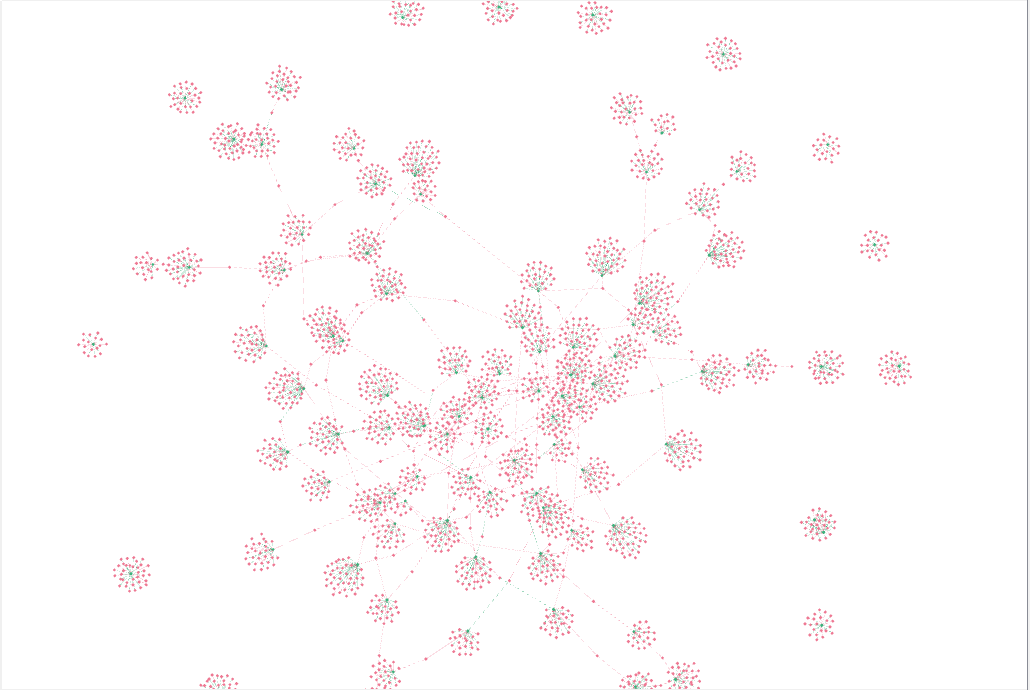
\includegraphics[width=.6\linewidth]{./graphs/CP_by_type.png}
        \caption{Company to People Graph. Red nodes represent people and green nodes represent companies}
    \end{figure}\\
    \textbf{CP Graph Construction (Figure 1)}\\
    A multi-directed, bipartite graph was constructed with two node types: companies and people. There was a directed edge drawn from a given company to every person employed as part of that's company senior management. Furthermore, every edge directed towards a CEO was given a weight of $2$ while every other edge directed toward an exec member had a weight of $1$. In addition there was a directed edge drawn from every member of the board of directors to the company they represent. For members who held a Chairman position on the board, a weight of $2$ was assigned whereas for members who held Vice Chair or Lead Director position, a weight of $1.5$ was assigned. For general board members, a weight of $1$ was assigned. This network had 2947 nodes, 2847 of which were people, and 3159 edges.\\
    \begin{figure}[h]
        \centering
        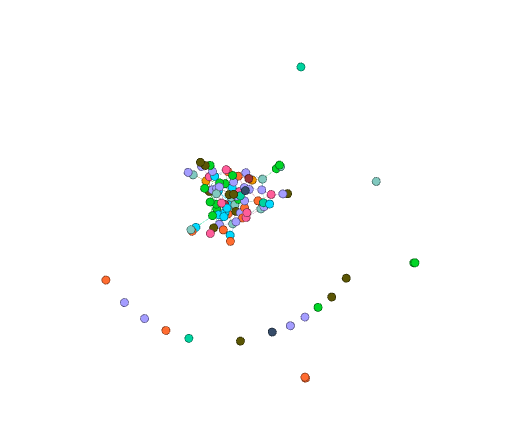
\includegraphics[width=.6\linewidth]{./graphs/CC_by_industry.png}
        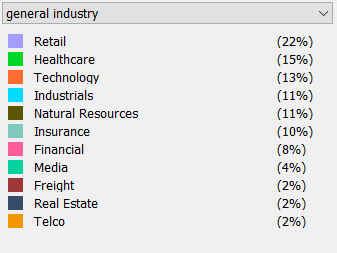
\includegraphics[width=.35\linewidth]{./graphs/CC_by_industry_legend.png}
        \caption{Company to Company Graph}
    \end{figure}\\
    \textbf{CC Graph Construction (Figure 2)}\\
    An undirected graph was constructed connecting companies through the people they share. Regardless of senior management employment or board membership, an edge was drawn between two companies that shared at least one person. Furthermore, this edge was weighted with the number of people shared between the two companies. In addition, company industries were added in the visualization in \textit{Figure 2}. This network had 100 nodes and 160 edges. 

\section*{Results and Discussion}

\subsection*{Company to People Graph}
\begin{figure}[h]
    \centering
    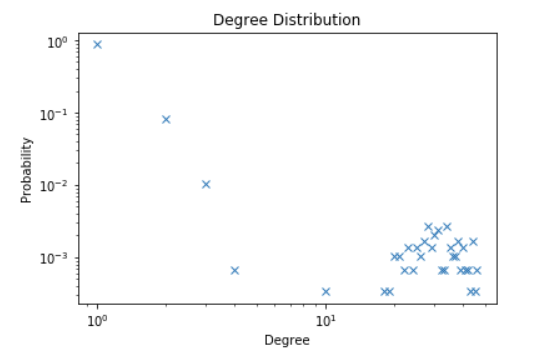
\includegraphics[width=.55\linewidth]{./graphs/CP_deg_dist_loglog.png}
    \caption{Log-log plot of the degree distribution for the CP graph}
\end{figure}
The average degree of nodes in the CP graph is 2.144. This makes sense since most people in the graph will have roughly 1 to 3 connections and the number of people greatly outweighs the number of companies. Looking at the degree distribution in \textit{Figure 3} we can see all of these results as there is a high probability that a node has a small degree. There is also a cluster of points to the bottom right of the graph signaling that there are a few nodes with a high degree. These are most likely companies since, as was discussed before, the average number of members on the board is 11.68 and the average number of people employed as senior management is 19.91. \par
\begin{figure}[h]
    \centering
    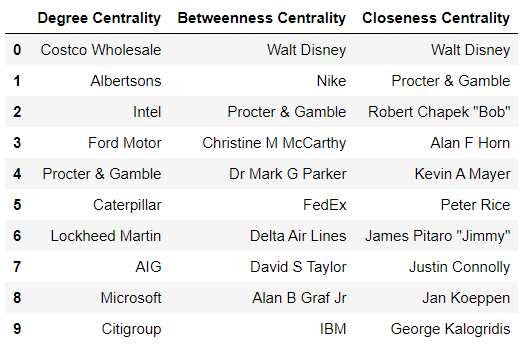
\includegraphics[width=.5\linewidth]{./graphs/centrality_CP.png}
    \caption{Top 10 nodes by each centrality measure. First is highest score for the given centrality measure}
\end{figure}
As we can see from \textit{Figure 4}, companies have the largest degree centrality. This matches the assumption from our degree distribution that companies generally have a much higher degree than people due to companies having multiple members on both the executive board and board of directors. However, we see that when ranking nodes by betweenness centrality and closeness centrality, people also have high centrality values. This is due to the possibility of people to serve as bridges between companies or for them to be linked to a more central company. For example, we see that when it comes to closeness centrality, Walt Disney and Procter and Gamble are the only companies that are on the list of top ten nodes by closeness centrality. All of the other individuals listed are executives at Walt Disney or one of its subsidiaries. 

\subsection*{Company to Company Graph}
\begin{figure}[h]
    \centering
    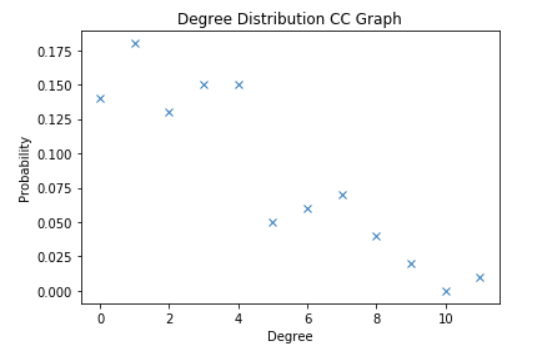
\includegraphics[width=.55\linewidth]{./graphs/deg_dist_CC.png}
    \caption{Plot of the degree distribution for the CC graph}
\end{figure}
The average degree of the nodes in the CC graph is 3.2. Looking at the degree distribution in \textit{Figure 5} we can see that there is an inverse relationship between the number of nodes and the degree. This is understandable considering that very few companies have a high number of linkages with other companies through common members of their board of directors or senior management employees.
\begin{figure}[h]
    \centering
    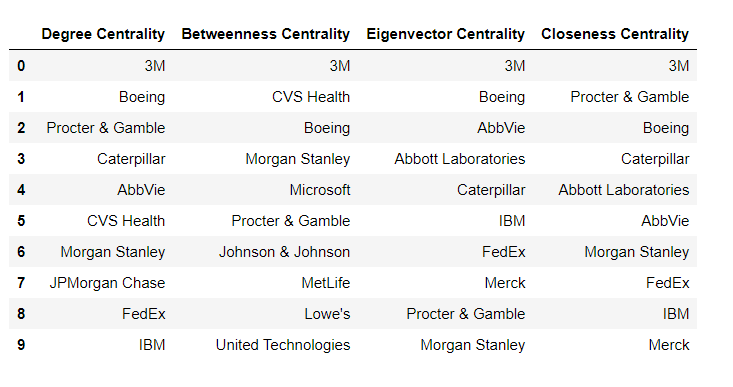
\includegraphics[width=.5\linewidth]{./graphs/centrality_CC.png}
    \caption{Top 10 nodes by each centrality measure. First is highest score for the given centrality measure}
\end{figure}
As we can see from \textit{Figure 6}, 3M dominates the lists for all four centrality measures. Furthermore, we see that many of the top 10 companies by degree centrality tend to also dominate across all the other centrality measures. Taking a deeper dive into 3M, we see that some of their senior management employees serve on the board of directors at companies including IBM, Allstate, Microsoft, and Proctor and Gamble. In total, their senior management employees serve on the board of directors of eleven of the top 100 US publicly traded companies. 
\par 
Furthermore, we took a look at the assortativity across industry for the CC graph. The assortativity coefficient of the CC graph was $-0.0355$. This suggests disassortative mixing in the CC graph. This makes sense since companies would want to avoid influence from individuals who are working for their competitors in the same industry. By having members of the board of directors come from senior management personnel in different industries or individuals in the private sector, companies avoid possible conflicts of interest from competitors. Furthermore, having members involved in other industries enables companies to forge meaningful relationships with other companies that they do not directly compete with. One notable example was Steve Jobs (then Apple CEO) and Bob Iger (Disney CEO) serving on the board of directors of the other company. During their terms, Disney was the first to be able to offer full-length TV shows on iTunes, and they partnered together for Disney's \#DreamBigPrincess campaign, among other things. However, Bob Iger resigned from Apple's board of directors in 2019 when both Disney and Apple launched streaming services, making the companies direct competitors with each other. 

\newpage
\section*{Conclusion}
It is apparent by the network analysis conducted above that the Fortune 100 are indeed well-connected through their board of directors and senior management employees. However, the extent of the overlap is often very small which means that there are a few individuals who act as bridges between companies as opposed to extensive overlapping boards. This phenomenon is not constrained to any particular industry and in fact, we see that often times companies who are not in the same industry are linked through their boards of directors and senior management employees.
    \subsection*{Further Analysis}
    There is a multitude of further analysis that can be conducted to build off of the work done in this paper. A larger data set, the Fortune 500, could be looked at to strengthen the analysis and provide more evidence for the conclusions that were drawn. Also expanding the data set to include international companies and then comparing by region would better give a sense of the interconnectedness in different national economies. Lastly, further work could also look deeper into the root cause of overlaps between companies to see what is actually motivating the interconnectedness.

\section*{GitHub Link}
Link: \url{https://github.com/aneespatwa/cse416_fl2019_finalProject_AneesPatwa_ChenthuranAbeyakaran/}

\nocite{*}
\bibliography{references}
\bibliographystyle{ieeetr}

\end{document}